\chapter{Resultados}\label{chapter:results}

En esta sección presentamos los resultados obtenidos. Nuestro enfoque se centró en la exploración y optimización de dos pipelines de procesamiento y clasificación de imágenes. Los experimentos se estructuraron con el objetivo de evaluar mejoras de precisión en el modelo utilizando distintas aproximaciones de división y normalización de datos en el contexto del procesamiento de imágenes.

El modelo con mayor eficiencia luego de varios ajustes tuvo una eficacia de validación cercana al 84\%. Los resultados son un paso significativo hacia la automatización del diagnóstico del cáncer de piel, que tradicionalmente ha dependido de la inspección visual por parte de expertos humanos. 

En cada sección se muestran algunas métricas que muestran el desarrollo del modelo, con los siguientes parámetros:

\begin{table}[ht]
   \centering
   \small
   \begin{tabular}{|c|p{10cm}|}
   \hline
   \textbf{Término} & \textbf{Descripción} \\
   \hline
   Epoch & Es una iteración completa sobre todo el conjunto de datos de entrenamiento. \\
   \hline
   Loss (Pérdida) & Es una medida de cuán bien el modelo está realizando sus predicciones. Los valores decrecientes indican una mejora en el aprendizaje. \\
   \hline
   Accuracy (Precisión) & Muestra el porcentaje de etiquetas que el modelo predice correctamente para el conjunto de entrenamiento. \\
   \hline
   V loss (Pérdida de Validación) & Es similar a la pérdida, pero se calcula sobre un conjunto de datos que no se utiliza para el entrenamiento. \\
   \hline
   V acc (Precisión de Validación) & Muestra el porcentaje de etiquetas que el modelo predice correctamente para el conjunto de datos de validación. \\
   \hline
   LR (Learning Rate) & La tasa de aprendizaje dicta cuánto se ajustan los pesos del modelo en cada actualización. \\
   \hline
   Next LR (Próxima Learning Rate) & Indica la próxima tasa de aprendizaje planificada. La adaptación de la tasa de aprendizaje puede ayudar a evitar el estancamiento y mejorar la convergencia. \\
   \hline
   Monitor & Muestra la métrica que se está utilizando para monitorizar el rendimiento del modelo. Cambia de \textit{accuracy} a \textit{val loss}, lo que probablemente indica que el cambio se hizo para evitar el sobre'ajuste. \\
   \hline
   Duration (Duración) & Tiempo que tardó cada epoch en completarse. Importante para evaluar la eficiencia del entrenamiento. \\
   \hline
   \end{tabular}
   \caption{Descripción de términos clave en el entrenamiento de modelos de aprendizaje automático.}
   \label{table:terminology}
   \end{table}
   

\section{Experimento 1: Evaluación de la eficiencia de la división asimétrica de datos en la clasificación de imágenes de cáncer de piel}\label{subsec:exp1}


%-----------------------------------------------------------------------------------
\subsection*{Estadísticas básicas}\label{sub:basic_statistics_p1}
%-----------------------------------------------------------------------------------
    
    Estos resultados de la tabla siguiente corresponden a la evaluación del modelo a lo largo de 40 epochs (iteraciones) de entrenamiento.

    \begin{figure}[ht]
      \small
      \begin{center}
          \begin{tabular}{|c|c|c|c|c|c|c|c|} \hline
          E & Loss & Acc & V loss & V acc & LR & M & Batch \\ \hline
          1 & 9.587 & 40.581 & 8.95658 & 56.800 & $10^{-2}$ & accuracy & 85.25 \\ \hline
          2 & 7.798 & 67.615 & 7.67235 & 66.800 & $10^{-2}$ & accuracy & 21.72 \\ \hline
          3 & 6.884 & 79.340 & 6.96014 & 69.600 & $10^{-2}$ & accuracy & 22.56 \\ \hline
          4 & 6.214 & 87.365 & 6.35865 & 71.200 & $10^{-2}$ & accuracy & 25.81 \\ \hline
          5 & 5.646 & 91.690 & 5.94812 & 75.200 & $10^{-2}$ & val\_loss & 23.08 \\ \hline
          6 & 5.172 & 92.999 & 5.44954 & 76.800 & $10^{-2}$ & val\_loss & 23.23 \\ \hline
          7 & 4.735 & 94.479 & 5.06016 & 76.400 & $10^{-2}$ & val\_loss & 23.19 \\ \hline
          8 & 4.334 & 96.528 & 4.73837 & 76.800 & $10^{-2}$ & val\_loss & 22.90 \\ \hline
          9 & 3.969 & 97.211 & 4.33689 & 77.200 & $10^{-2}$ & val\_loss & 22.74 \\ \hline
          10 & 3.631 & 98.008 & 4.15826 & 74.000 & $10^{-2}$ & val\_loss & 22.56 \\ \hline
          11 & 3.315 & 98.406 & 3.89153 & 73.600 & $10^{-2}$ & val\_loss & 23.11 \\ \hline
          \dots & \dots & \dots & \dots & \dots & \dots & \dots & \dots \\ \hline
          34 & 0.627 & 99.886 & 1.24470 & 76.800 & 0.00013 & val\_loss & 23.30 \\ \hline
          \end{tabular}
          \caption{Estadísticas básicas del modelo EfficientNetB1.}
      \end{center}\label{fig:estadisticas_p1}
  \end{figure}
    
  Aquí vemos que el entrenamiento se planeó para 40 epochs, pero se detuvo en el epoch 34, después de tres ajustes de la tasa de aprendizaje sin mejoras en la pérdida de validación. Esto ocurre dado que el modelo no estaba mejorando su capacidad de generalizar a datos no vistos y que continuar el entrenamiento probablemente habría resultado en un gasto innecesario de recursos y posiblemente en un mayor sobre-ajuste. 
  
  En la tabla se observa que la precisión de entrenamiento aumenta con cada epoch, la pérdida de entrenamiento disminuye consistentemente, la tasa de aprendizaje permanece constante al principio y luego disminuye para afinar el entrenamiento a medida que el modelo comienza a converger, todo lo anterior es indicador que el modelo esta entrenando de forma correcta.

  En el monitor se muestra que cambia de \textit{accuracy} a \textit{val loss}, este cambio se hizo para evitar el sobre-ajuste.

%-----------------------------------------------------------------------------------
\subsection*{Estadísticas de aprendizaje}\label{sub:learning_statistics_p1}
%-----------------------------------------------------------------------------------
		\begin{figure}[ht]%
      \begin{center}
      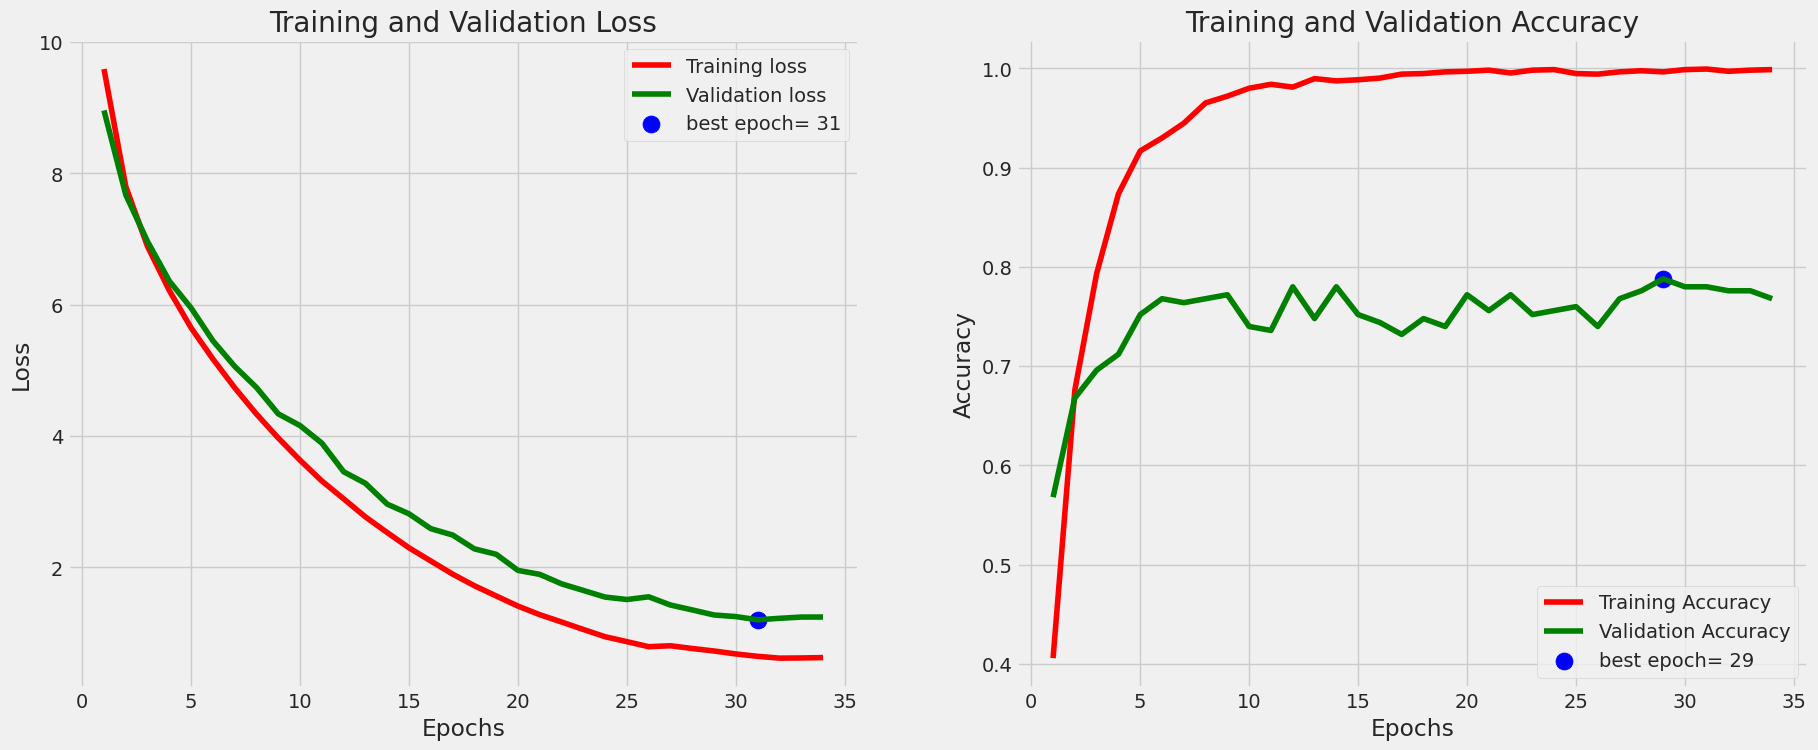
\includegraphics[width=1\textwidth]{./Graphics/training&validation_p1.png}
      \caption{Estadísticas de aprendizaje a lo largo del proceso de entrenamiento.\label{fig:training_validation_loss}}
      \end{center}
		\end{figure}
  
La imagen anterior muestra dos gráficos, uno de pérdida y otro de precisión respectivamente, a lo largo de los epochs de entrenamiento y validación. El primero muestra una disminución constante de la pérdida tanto en el entrenamiento como en la validación, lo cual es indicativo de un buen aprendizaje. La pérdida de validación tiene un mínimo en el epoch 31, lo que sugiere que este podría ser el mejor modelo para evitar el sobre-ajuste. A partir de este punto, si la pérdida de validación comenzase a aumentar mientras la pérdida de entrenamiento sigue disminuyendo, indicaría sobre-ajuste.

En el segundo se aprecia como la precisión de entrenamiento aumenta rápidamente y luego se estabiliza cerca del 100\%, mientras que la precisión de validación también aumenta pero con cierta variabilidad entre los epochs. El mejor epoch según la precisión de validación es el 29. Esta diferencia entre la precisión de entrenamiento y de validación sugiere que puede haber variabilidad en los datos de validación.

%-----------------------------------------------------------------------------------
\subsection*{Estadísticas de eficacia}\label{sub:accuracy_statistic_p1}
%-----------------------------------------------------------------------------------
\begin{figure}[ht]%
   \begin{center}
   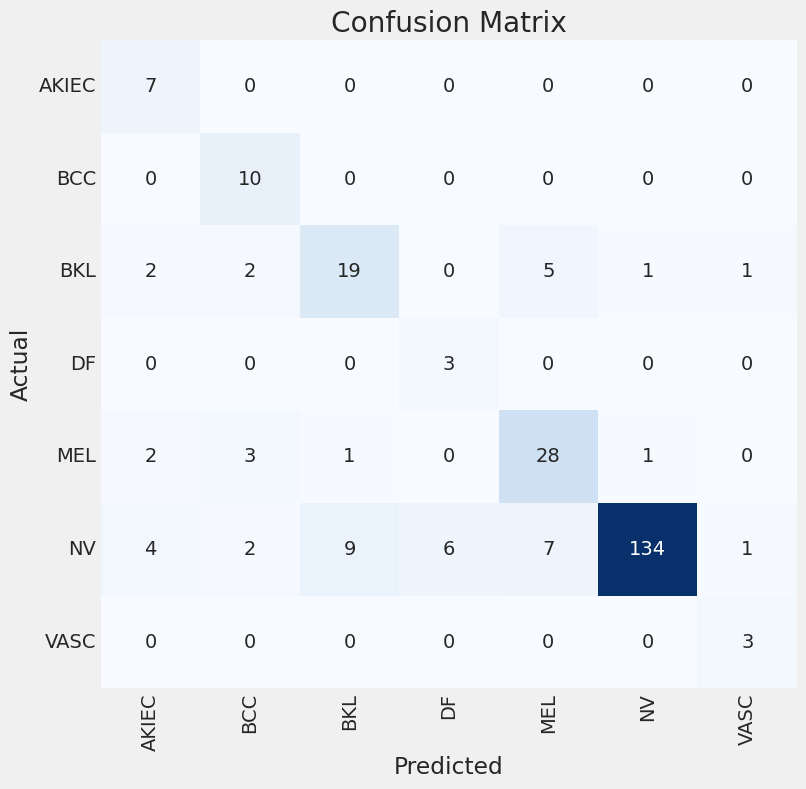
\includegraphics[width=0.8\textwidth]{./Graphics/confussionmatrix_p1.png}
   \caption{Estadísticas de eficacia del modelo al estimar los resultados en el conjunto de pruebas\label{fig:confussion_matrix_p1}}
   \end{center}
   \end{figure}

   \begin{figure}[ht]%
      \begin{center}
      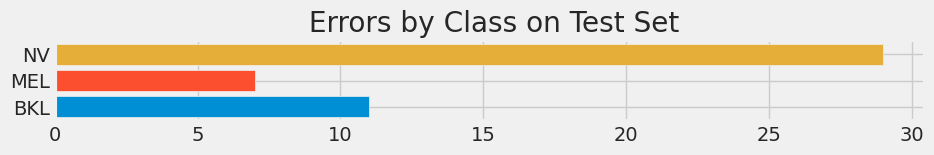
\includegraphics[width=0.8\textwidth]{./Graphics/errorByClass_p1.png}
      \caption{Gráfico de errores por clase en el conjunto de pruebas\label{fig:class_errors_p1}}
      \end{center}
      \end{figure} 


La matriz de confusión proporciona información valiosa sobre el rendimiento del modelo en relación de Actual/Predicho, en términos de su capacidad para clasificar correctamente cada una de las siete clases de cáncer de piel. La diagonal principal de la matriz representa los verdaderos positivos (TP), el número de casos en los que el modelo ha predicho correctamente la clase correspondiente. Los valores fuera de la diagonal principal indican errores de clasificación.

    La clase 'NV' muestra una alta cantidad de clasificaciones correctas (134), pero también tiene errores significativos al ser confundida con otras clases (como 'BKL' y 'MEL'). La clase 'AKIEC' resultó la más difícil de predecir, con la mayoría de las muestras mal clasificadas. Esto puede deberse a la similitud entre las características de estas clases, pero sobre todo al desbalance en el conjunto de datos.
    
    Cada barra representa el número de muestras de una clase particular que fueron mal clasificadas.

\subsection*{Informe de clasificación}

\begin{table}[ht]
    \centering
    \caption{Informe de clasificación para el Experimento 1}
    \label{tab:classification_report_exp1}
    \begin{tabular}{lcccc}
    \hline
    \textbf{Categoría Diagnóstica} & \textbf{Precisión} & \textbf{Recall} & \textbf{F1-Score} & \textbf{Soporte} \\
    \hline
    AKIEC & 0.47 & 1.00 & 0.64 & 7 \\
    BCC   & 0.59 & 1.00 & 0.74 & 10 \\
    BKL   & 0.66 & 0.63 & 0.64 & 30 \\
    DF    & 0.33 & 1.00 & 0.50 & 3 \\
    MEL   & 0.70 & 0.80 & 0.75 & 35 \\
    NV    & 0.99 & 0.82 & 0.90 & 163 \\
    VASC  & 0.60 & 1.00 & 0.75 & 3 \\
    \hline
    \textbf{Accuracy} & & & 0.81 & 251 \\
    \textbf{Macro Avg} & 0.62 & 0.89 & 0.70 & 251 \\
    \textbf{Weighted Avg} & 0.86 & 0.81 & 0.83 & 251 \\
    \hline
    \end{tabular}
    \end{table}

Resultados Generales: La precisión global del modelo fue del 81\%, con una media ponderada de precisión del 86\%, recall del 81\%, y una puntuación F1 del 83\%.
Resultados por Categoría Diagnóstica: Describir la precisión, el recall, y la puntuación F1 para cada categoría diagnóstica, destacando que 'NV' tuvo la precisión más alta (0.99) y 'AKIEC' la más baja (0.47). El recall fue perfecto (1.00) para 'AKIEC', 'BCC', 'DF', y 'VASC', lo que indica que todas las muestras verdaderas fueron identificadas correctamente, pero la precisión varió, sugiriendo un posible desequilibrio en la identificación de falsos positivos.

\section{Experimento 2: Análisis de la estratificación de datos en la clasificación de imágenes de cáncer de piel}

%-----------------------------------------------------------------------------------
\subsection*{Estadísticas básicas}\label{sub:basic_statistics_p2}
%-----------------------------------------------------------------------------------
    
    Estos resultados de la tabla siguiente corresponden a la evaluación del modelo a lo largo de 40 epochs (o iteraciones) de entrenamiento. Cada fila representa una época y se presentan las siguientes métricas:
    
    \begin{figure}[ht]
      \small
      \begin{center}
          \begin{tabular}{|c|c|c|c|c|c|c|c|} \hline
          E & Loss & Acc & V loss & V acc & LR & M & Batch \\ \hline
          1 & 9.587 & 40.581 & 8.95658 & 56.800 & $10^{-2}$ & accuracy & 85.25 \\ \hline
          2 & 7.798 & 67.615 & 7.67235 & 66.800 & $10^{-2}$ & accuracy & 21.72 \\ \hline
          3 & 6.884 & 79.340 & 6.96014 & 69.600 & $10^{-2}$ & accuracy & 22.56 \\ \hline
          4 & 6.214 & 87.365 & 6.35865 & 71.200 & $10^{-2}$ & accuracy & 25.81 \\ \hline
          5 & 5.646 & 91.690 & 5.94812 & 75.200 & $10^{-2}$ & val\_loss & 23.08 \\ \hline
          6 & 5.172 & 92.999 & 5.44954 & 76.800 & $10^{-2}$ & val\_loss & 23.23 \\ \hline
          7 & 4.735 & 94.479 & 5.06016 & 76.400 & $10^{-2}$ & val\_loss & 23.19 \\ \hline
          8 & 4.334 & 96.528 & 4.73837 & 76.800 & $10^{-2}$ & val\_loss & 22.90 \\ \hline
          9 & 3.969 & 97.211 & 4.33689 & 77.200 & $10^{-2}$ & val\_loss & 22.74 \\ \hline
          10 & 3.631 & 98.008 & 4.15826 & 74.000 & $10^{-2}$ & val\_loss & 22.56 \\ \hline
          11 & 3.315 & 98.406 & 3.89153 & 73.600 & $10^{-2}$ & val\_loss & 23.11 \\ \hline
          \dots & \dots & \dots & \dots & \dots & \dots & \dots & \dots \\ \hline
          34 & 0.627 & 99.886 & 1.24470 & 76.800 & 0.00013 & val\_loss & 23.30 \\ \hline
          \end{tabular}
          \caption{Estadísticas básicas de algunas iteraciones del modelo EfficientNetB1.}
      \end{center}\label{fig:estadisticas_p2}
  \end{figure}
    
    En general, los resultados muestran que el modelo mejora con el tiempo, ya que la pérdida disminuye y la precisión aumenta tanto en el conjunto de datos de entrenamiento como en el de validación.

%-----------------------------------------------------------------------------------
\subsection*{Estadísticas de aprendizaje}\label{sub:learning_statistics_p2}
%-----------------------------------------------------------------------------------
		\begin{figure}[ht]%
      \begin{center}
      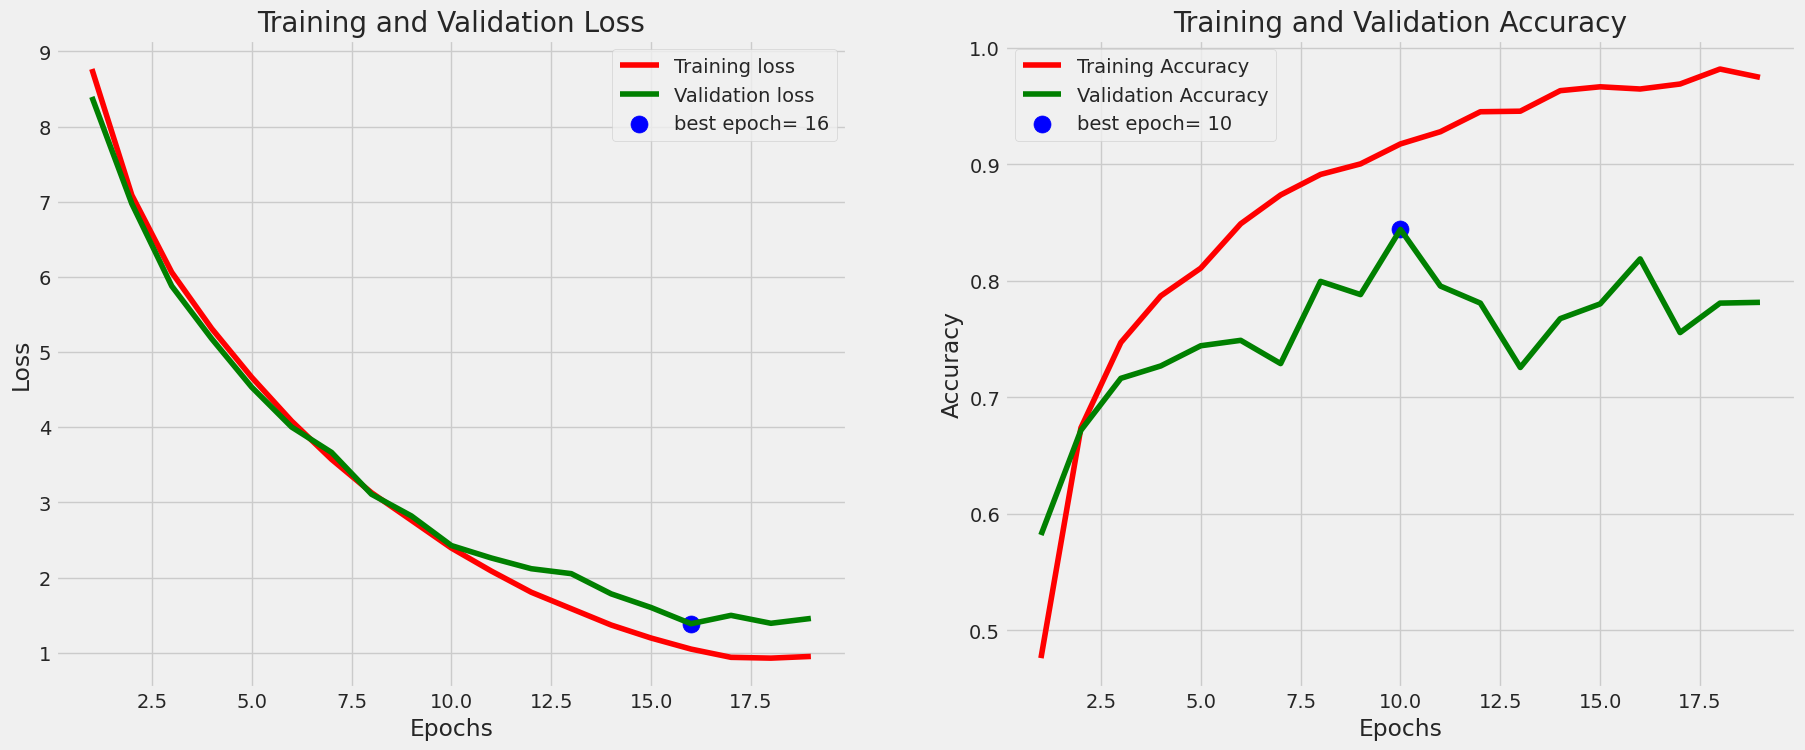
\includegraphics[width=1\textwidth]{./Graphics/training&validation_p2.png}
      \caption{Estadísticas de aprendizaje a lo largo del proceso de entrenamiento.\label{fig:training_validation_loss_p2}}
      \end{center}
		\end{figure}
  
La época con la mejor pérdida de validación y la mejor precisión de validación no coinciden, sugiere un trade-off entre la optimización de la pérdida y la maximización de la precisión. La volatilidad en la precisión de validación sugiere que el modelo puede beneficiarse de un ajuste en el tamaño del lote para suavizar las actualizaciones de los pesos y mejorar la estabilidad del modelo.

Dado lo anterior, se hizo una última iteración del modelo aumentando el volumen de muestras por clase a 500. Estos fueron los resultados. Se obtuvo una efectividad de aproximadamente 87\% (86.83\%).

\begin{figure}[ht]%
   \begin{center}
   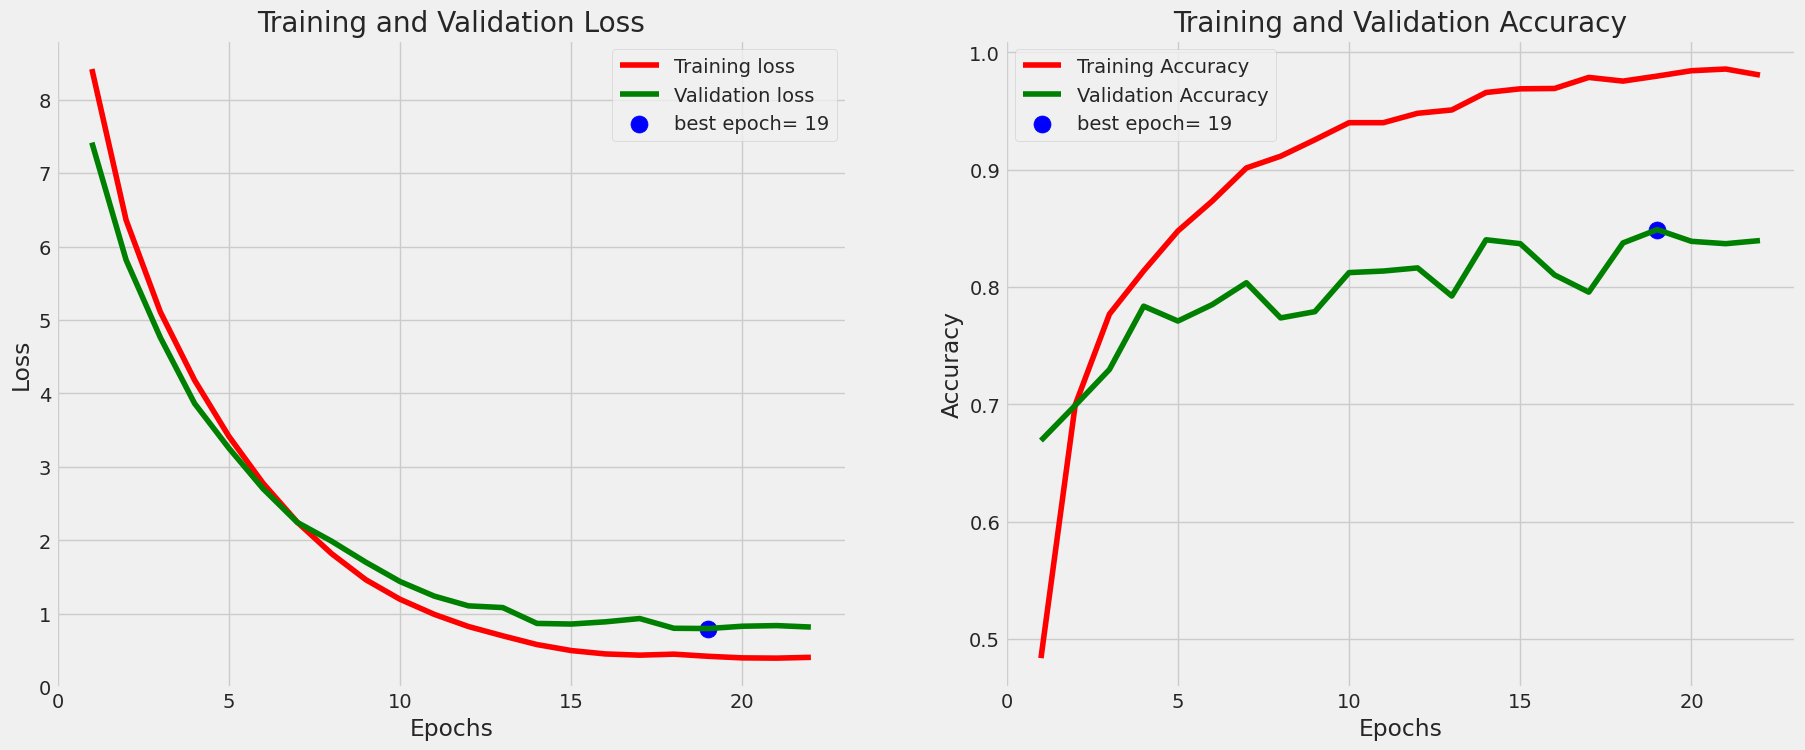
\includegraphics[width=1\textwidth]{./Graphics/training&validation_p3.png}
   \caption{Estadísticas de aprendizaje a lo largo del proceso de entrenamiento.\label{fig:training_validation_loss_p3}}
   \end{center}
   \end{figure}

La disminución continua en la pérdida de entrenamiento y la tendencia ascendente en la precisión de entrenamiento sugieren que el modelo está aprendiendo de manera efectiva y consistente. La pérdida de validación que converge con la de entrenamiento y la mejor época coincidente para pérdida y precisión de validación (época 19) indican que el modelo generaliza bien y no solo memoriza los datos de entrenamiento.

En el gráfico actual, hay una mejor alineación entre la pérdida de entrenamiento y validación y menos volatilidad en la precisión de validación, lo que indica un modelo más estable.

%-----------------------------------------------------------------------------------
\subsection*{Estadísticas de eficacia}\label{sub:accuracy_statistic_p2}
%-----------------------------------------------------------------------------------
    
\begin{figure}[ht]%
   \begin{center}
   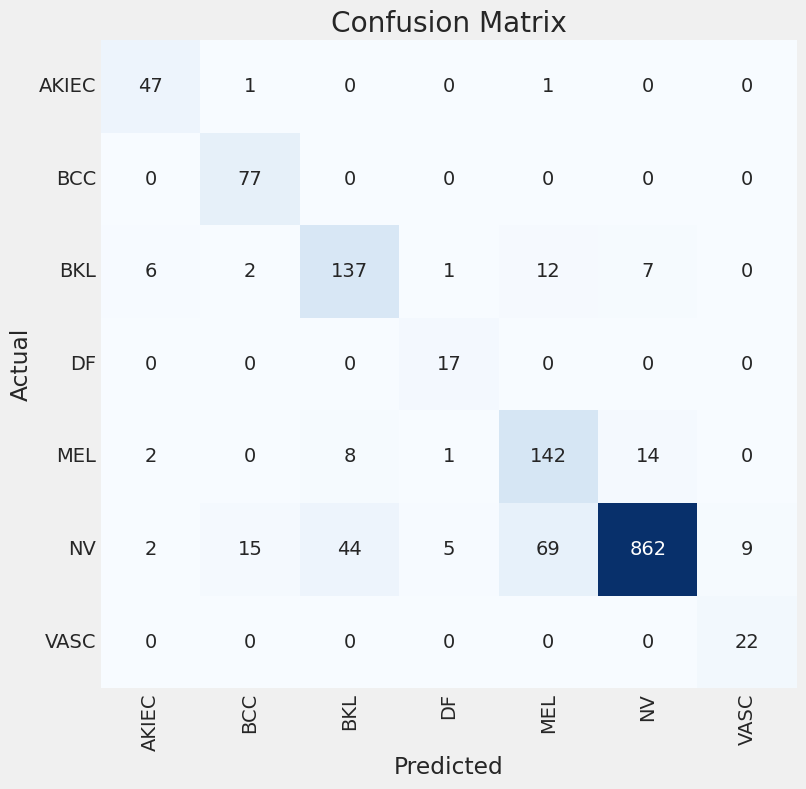
\includegraphics[width=0.8\textwidth]{./Graphics/confussionMatrix_p3.png}
   \caption{Estadísticas de eficacia del modelo al estimar los resultados en el conjunto de pruebas\label{fig:confussion_matrix_p3}}
   \end{center}
   \end{figure}

   \begin{figure}[ht]%
      \begin{center}
      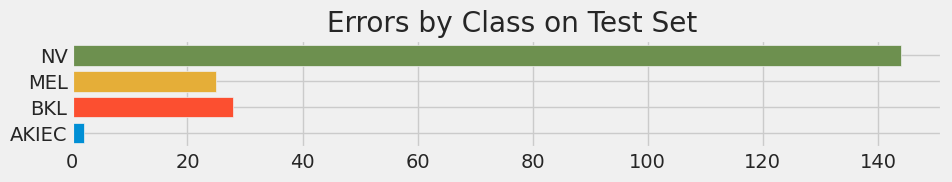
\includegraphics[width=0.8\textwidth]{./Graphics/errorByClass_p3.png}
      \caption{Gráfico de errores por clase en el conjunto de pruebas\label{fig:class_errors_p3}}
      \end{center}
      \end{figure}

NV muestra la mayoría de los errores, lo que puede deberse a una mayor prevalencia en el conjunto de datos.

Comparando ambos gráficos, podemos identificar áreas específicas donde el modelo necesita mejora. Por ejemplo, la clase 'NV', a pesar de tener muchas predicciones correctas, tiene un número relativamente alto de falsos positivos y falsos negativos, lo que sugiere que puede haber características de las imágenes 'NV' que se confunden con otras clases. En cambio, 'BCC' y 'DF' parecen estar bien diferenciados del resto. Esto puede informar estrategias futuras para mejorar la precisión del modelo, como la recolección de más datos o la implementación de técnicas de aprendizaje más avanzadas para clases específicas.

\subsection*{Informe de clasificación}

    
    \begin{table}[H]
        \centering
        \caption{Informe de clasificación para el Experimento 2}
        \label{tab:classification_report_exp2}
        \begin{tabular}{lcccc}
        \hline
        \textbf{Categoría Diagnóstica} & \textbf{Precisión} & \textbf{Recall} & \textbf{F1-Score} & \textbf{Soporte} \\
        \hline
        AKIEC & 0.82 & 0.96 & 0.89 & 49 \\
        BCC   & 0.81 & 1.00 & 0.90 & 77 \\
        BKL   & 0.72 & 0.83 & 0.77 & 165 \\
        DF    & 0.71 & 1.00 & 0.83 & 17 \\
        MEL   & 0.63 & 0.85 & 0.73 & 167 \\
        NV    & 0.98 & 0.86 & 0.91 & 1006 \\
        VASC  & 0.71 & 1.00 & 0.83 & 22 \\
        \hline
        \textbf{Accuracy} & & & 0.87 & 1503 \\
        \textbf{Macro Avg} & 0.77 & 0.93 & 0.84 & 1503 \\
        \textbf{Weighted Avg} & 0.89 & 0.87 & 0.87 & 1503 \\
        \hline
        \end{tabular}
        \end{table}
        
Resultados Generales: La precisión global del modelo fue del 87\%, con una media ponderada de precisión del 89\%, recall del 87\%, y una puntuación F1 del 87\%.
Resultados por Categoría Diagnóstica: Enumerar la precisión, el recall, y la puntuación F1 para cada categoría diagnóstica. Resalta que todas las categorías mejoraron en comparación con el Experimento 1, con 'NV' mostrando nuevamente la precisión más alta (0.98) y 'MEL' la más baja (0.63).



\section{Comparación entre los Experimentos}\label{subsubsec:comparison_exp}
%-----------------------------------------------------------------------------------

Eficiencia del Modelo: El Experimento 2 demuestra una eficiencia general superior con una mayor precisión de validación y un modelo más estable. Esto puede atribuirse a un balance más efectivo de clases y a ajustes en la tasa de aprendizaje.

Manejo de Desequilibrio de Clases: El Experimento 2 maneja mejor el desequilibrio de clases, lo que se refleja en una mejor diferenciación entre ciertas categorías diagnósticas.

Generalización: El Experimento 2 muestra una tendencia más estable en la pérdida de validación y en la precisión, sugiriendo una mejor capacidad para generalizar a nuevos datos.

Implicaciones para la Clasificación de Cáncer de Piel: Estos resultados resaltan la importancia de la estratificación de datos y del balance de clases en la clasificación de imágenes médicas, especialmente en contextos donde la variabilidad entre categorías es significativa.

\subsection{Comparación de Ventajas y Desventajas}

Ventajas del Experimento 1
\begin{enumerate}
    \item Sensibilidad: El modelo del Experimento 1 demostró una alta sensibilidad, con un recall perfecto en varias categorías, lo que es crucial en aplicaciones médicas para evitar falsos negativos.
    \item Eficiencia en Categorías Específicas: Ciertas categorías como 'NV' tuvieron una precisión extremadamente alta, lo que sugiere una eficiencia notable en la identificación de esta condición común.
\end{enumerate}

Desventajas del Experimento 1
\begin{enumerate}
    \item Balance de Precisión-Recall: Aunque el modelo tenía un alto recall en algunas categorías, la precisión era baja, lo que podría resultar en un número más alto de falsos positivos.
    \item Consistencia en el Rendimiento: La variabilidad en el rendimiento entre categorías puede indicar una necesidad de ajustar el modelo o los datos para mejorar la consistencia.
\end{enumerate}

Ventajas del Experimento 2
\begin{enumerate}
    \item Mejora en Precisión y F1-Score: El modelo del Experimento 2 mostró mejoras en la precisión y puntuación F1 en todas las categorías, indicando un equilibrio más sólido entre la precisión y el recall.
    \item Rendimiento General: Con una precisión global y una puntuación F1 más altas que el Experimento 1, este modelo demostró ser más robusto y equilibrado.
\end{enumerate}

Desventajas del Experimento 2
\begin{enumerate}
    \item Potencial Sobreajuste: A pesar de la mejora en los indicadores, un rendimiento demasiado alto en el conjunto de entrenamiento podría sugerir un sobreajuste, especialmente si no se replica en datos independientes.
\end{enumerate}

\section{Consideraciones Finales}\label{subsubsec:final_considerations}
%-----------------------------------------------------------------------------------

Los resultados obtenidos son prometedores y sugieren que los modelos de aprendizaje profundo tienen un potencial considerable para mejorar la precisión y la eficiencia del diagnóstico del cáncer de piel
